\chapter{Z ve S tanım bölgesi}
Zaman tanım bölgesinden S tanım gölgesine dönüşüm
\begin{equation}
\begin{split}
    F(s)&=\mathcal{L}\{f(t)\}=\sum_{k=0}^{\infty}f(kT)e^{-kTs}\\
    &=f(0)+f(T)e^{-Ts}+f(2T)e^{-2Ts}+\cdots
\end{split}
\end{equation}
olarak verilmiştir. Zaman tanım bölgesinden Z tanım bölgesine geçiş ise
\begin{equation}
    \begin{split}
        F(z)&=\mathcal{Z}\{f(t)\}=\sum_{k=0}^{\infty}f(kT)z^{-k}\\
        &=f(0)+f(T)z^{-1}+f(2T)z^{-2}+\cdots
    \end{split}
\end{equation}
şeklindedir. S ve Z tanım bölgesi dönüşümlerine dikkat edilirse
\begin{equation}
    \begin{split}
        \mathcal{L}\{f(t)\}&=\sum_{k=0}^{\infty}f(kT)(e^{Ts})^{-k}\\
        \mathcal{Z}\{f(t)\}&=\sum_{k=0}^{\infty}f(kT)z^{-k}
\end{split}
\end{equation}
ifadelerinden
\begin{equation}
    z=e^{sT}
\end{equation}
ilişkisi elde edilir.
Z dönüşümü için çizelge Çizelge~\ref{tbl:ztransform1} ile verilmiştir.
\begin{table}[!htb]
    \centering
    \caption{S ve Z dönüşümü tablosu}
    \label{tbl:ztransform1}
    \begin{tabular}{ccc}\hline
        Zaman domeni& $F(s)$& $F(z)$\\\hline
        $\delta(t)$& $1$& $1$\\
        $\delta(t-kT)$& $e^{-kTs}$& $z^{-k}$\\
        $u(t)=1$& $\frac{1}{s}$& $\frac{z}{z-1}$\\
        $t$& $\frac{1}{s^2}$& $\frac{Tz}{(z-1)^2}$\\
        $e^{-at}$& $\frac{1}{s+a}$& $\frac{z}{z-e^{-aT}}$\\
        $1-e^{-at}$& $\frac{a}{s(s+a)}$& $\frac{z(1-e^{-aT})}{(z-1)(z-e^{-aT})}$\\
        $sin(wt)$& $\frac{w}{s^2+w^2}$& $\frac{zsin(wT)}{(z-1)(z^2-2zcos(wT)+1)}$\\
        $cos(wt)$& $\frac{s}{s^2+w^2}$& $\frac{z(z-cos(wT))}{(z-1)(z^2-2zcos(wT)+1)}$\\\hline
    \end{tabular}
\end{table}
\begin{enumerate}
\item S dönüşümü
\begin{equation}
    \begin{split}
        \mathcal{L}\{1\}&=\int_{t=0}^{\infty}e^{-st}dt\\
        &=\frac{e^{-st}}{-s}\Bigg|_{t=0}^{\infty}\\
        &=\frac{e^{-s\infty}}{-s}-\frac{1}{-s}\\
        &=-\frac{1}{-s}\\
        &=\frac{1}{s}
    \end{split}
\end{equation}
olarak elde edilir. Z dönüşümü ise
\begin{equation}
    \begin{split}
        \mathcal{Z}\{1\}&=\sum_{t=0}^{\infty}z^{-t}\\
        &=1+z^{-1}+z^{-2}+z^{-3}+\cdots\\
        &=\frac{1}{1-z^{-1}},\quad |z|>1\\
        &=\frac{z}{z-1},\quad |z|>1\\
    \end{split}
\end{equation}
elde edilir.
\item \begin{equation}
    \int udv=uv-\int vdu
\end{equation}
kullanarak $u=t$ ve $dv=e^{-st}dt$ olmak üzere
\begin{equation}
    \begin{split}
        dv&=e^{-st}dt\\
        \int dv&=\int e^{-st}dt\\
        v&=\frac{e^{-st}}{-s}
    \end{split}
\end{equation}
ve dolayısıyla
\begin{equation}
    \begin{split}
        \mathcal{L}\{t\}&=\int_{t=0}^{\infty}t e^{-st}dt\\
        &=t\frac{e^{-st}}{-s}\Bigg|_{t=0}^{\infty}-\int_{t=0}^{\infty}\frac{e^{-st}}{-s}dt\\
        &=t\frac{e^{-st}}{-s}\Bigg|_{t=0}^{\infty}+\frac{1}{s}e^{-st}\Bigg|_{t=0}^{\infty}\\
        &=t\frac{e^{-st}}{-s}\Bigg|_{t=0}^{\infty}+\frac{1}{s^2}\\
        &=\frac{1}{s^2}
    \end{split}
\end{equation}
elde edilir. Z dönüşümü ise
\begin{equation}
    \begin{split}
        \sum_{t=0}^{\infty}t z^{t-1}&=1+2z+3z^2+4z^3+\cdots\\
        &=\frac{1}{(1-z)^2},\quad |z|<1
    \end{split}
\end{equation}
yardımıyla
\begin{equation}
    \begin{split}
        \mathcal{Z}\{t\}&=\sum_{t=0}^{\infty}tT (z^{-1})^{t}\\
        &=Tz^{-1}\sum_{t=0}^{\infty}t (z^{-1})^{t-1}\\
        &=T\frac{z^{-1}}{(1-z^{-1})^2},\quad |z|<1\\
        &=T\frac{\frac{1}{z}}{(1-\frac{1}{z})^2},\quad |z|<1\\
        &=T\frac{\frac{1}{z}}{\frac{(z-1)^2}{z^2}},\quad |z|<1\\
        &=T\frac{z^2}{z(z-1)^2},\quad |z|<1\\
        &=\frac{Tz}{(z-1)^2},\quad |z|<1
    \end{split}
\end{equation}
olarak elde edilir.
\end{enumerate}

\begin{enumerate}
    \item $sin(t)$ fonksiyonunu sürekli zaman ve ayrık zamanda çizdiriniz.
    \verb|Matlab| kodu
    \begin{lstlisting}[style=Matlab-editor]
    T=0.5;
    tvec=0:T:10;

    f1=@(t)sin(t);
    f1vec=f1(tvec);

    figure(1);clf;hold on;grid on;
    xlabel("Zaman(s)");ylabel("y(t)");title("sin(t) grafigi");
    plot(0:0.01:10,f1(0:0.01:10),'k','LineWidth',2);
    stem(tvec,f1(tvec),'r','LineWidth',2);
    \end{lstlisting}
    olarak verilmiştir. Şekil~\ref{fig:lec5_plot1} ile elde edilen grafik verilmiştir.
    \begin{figure}[!htb]
        \centering
        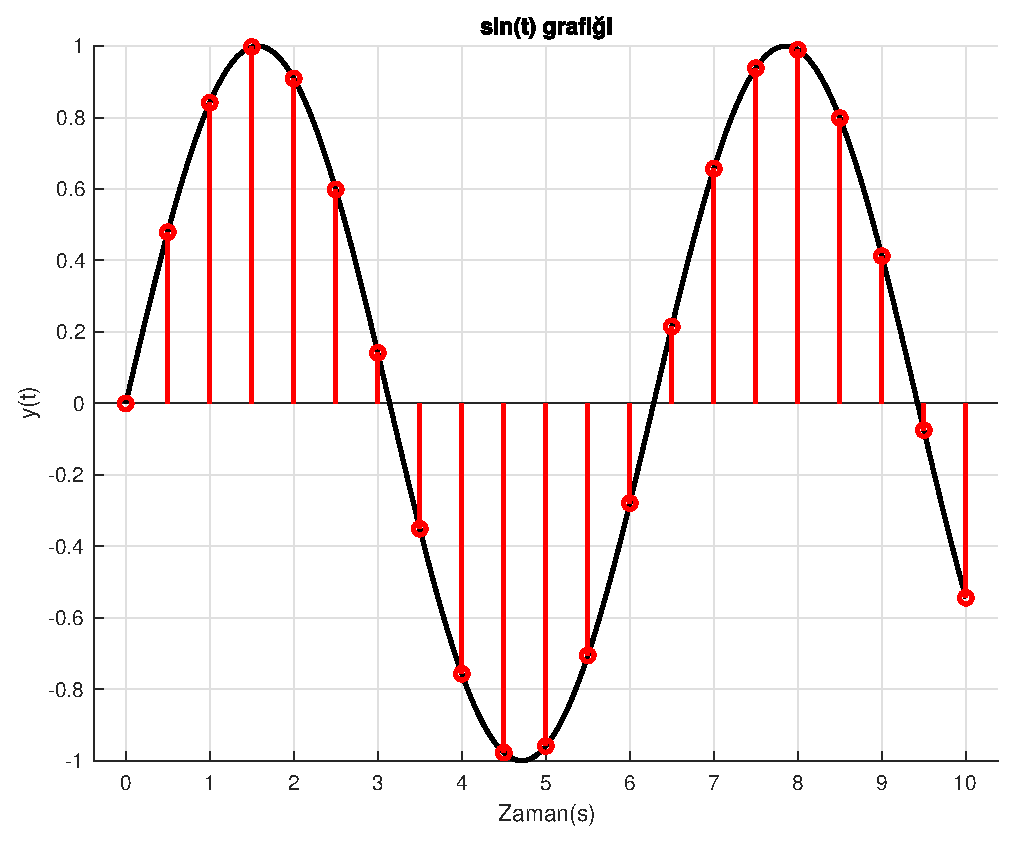
\includegraphics[width=0.5\textwidth]{img/lec5_plot1}
        \caption{$sin(t)$ sürekli zaman ve ayrık zaman karşılaştırması}
        \label{fig:lec5_plot1}
    \end{figure}
    \item $y=\delta(t)$ fonksiyonunun s tanım bölgesi ve z tanım bölgesi karşılığını elde ediniz.
    \begin{lstlisting}[style=Matlab-editor]
    syms t s z;
    yt=dirac(t);
    ys=laplace(yt);
    yz=ztrans(ys,s,z);
    \end{lstlisting}
    \item 
    \begin{equation}
        G(s)=\frac{2}{s^3+4s^2+5s+6}
    \end{equation}
    ifadesini basit kesir toplamına çeviriniz.
    \begin{lstlisting}[style=Matlab-editor]
    Gss=1/(s^3+4*s^2+5*s+6);
    expr=partfrac(Gss);
    pretty(expr)
    \end{lstlisting}
    \item $\int_{t=0}^{\infty} te^{-st}dt$ ifadesini hesaplayınız.
    \begin{lstlisting}[style=Matlab-editor]
    Gss=t*exp(-s*t);
    expr=int(Gss);
    subs(expr,t,inf)-subs(expr,t,0)
    \end{lstlisting}
\end{enumerate}